% Source: Weinberg GR, physical PDF pp. 320--322
%         (printed pp. 297--299).
% Coverage: Chapter 11 opening material before Section 11.1.
% Figures/tables/footnotes: chapter epigraph; Figure 11.1; no tables or
%                          footnotes.
% Status: source-reviewed and compile-clean.
% Uncertainties: none.

\begin{flushright}
\begin{minipage}{0.46\textwidth}
\itshape
``Things fall apart; the centre cannot hold,\\
Mere anarchy is loosed upon the world.''\\
W.~B. Yeats, \emph{The Second Coming}
\end{minipage}
\end{flushright}

Gravitational fields are so weak that the practicing astrophysicist can
usually ignore general relativity. This chapter deals with various sorts of
objects in which relativistic effects play an important, or, in some cases, a
dominant, role. One of these is the neutron star, a ``cold'' star composed
primarily of neutrons and supported against collapse by neutron degeneracy
pressure. Another is the supermassive star, a giant object supported by
radiation pressure, in which general-relativistic effects can tip the balance
between stability and instability. Most impressive of all is the black hole,
a body caught in an inexorable gravitational collapse.

The existence of neutron stars and black holes was suggested in the 1930s on
purely theoretical grounds, chiefly through the work of J.~Robert Oppenheimer
and his collaborators. However, these exotic objects remained a textbook
curiosity until the 1960s, when the cooperative efforts of radio and optical
astronomers began to reveal a great many strange new things in the sky.

First came the quasi-stellar objects (QSOs), objects with starlike optical
images, often containing powerful compact radio sources, and with redshifts
\(\Delta\lambda/\lambda\) ranging from \(0.131\) to nearly \(3\).
(See Figure~\ref{fig:11.1}.) One can suppose three different sorts of
explanations for these redshifts: they can arise from a Doppler effect, caused
either by a local explosion or by the general cosmological recession of very
distant objects (see Chapter~14), or they can arise from powerful
gravitational fields within the objects themselves. In any case, it is likely
that general-relativistic effects will play an important role in the
explanation of the QSOs. If these objects are relatively near but moving at
relativistic velocities, then some source of energy must be found that could
convert mass into kinetic energy, with nearly \(100\%\) efficiency. If the
QSOs are at cosmological distances, then their apparent optical luminosity
indicates an absolute luminosity much greater than that of the largest
galaxies, so again a powerful new source of energy is required. Only
gravitational attraction seems to offer an adequate energy source, and for
this reason the discovery of the QSOs reawakened general interest in the
phenomenon of gravitational collapse. Finally, if the QSO redshifts are
gravitational, then these objects must be so highly compressed that their
structure would have to be understood in terms of general relativity rather
than Newtonian mechanics.

% Source: Weinberg GR, physical PDF p. 321 (printed p. 298).
% Coverage: Figure 11.1, four quasi-stellar objects.
% Status: source page extracted losslessly; photographs clipped independently
%         so that all four object labels remain complete; source-reviewed.
% Uncertainties: none.

\begingroup
\renewcommand{\thefigure}{11.1}
\begin{figure}[htbp]
  \centering
  \begin{tabular}{@{}c@{\hspace{1.5em}}c@{}}
    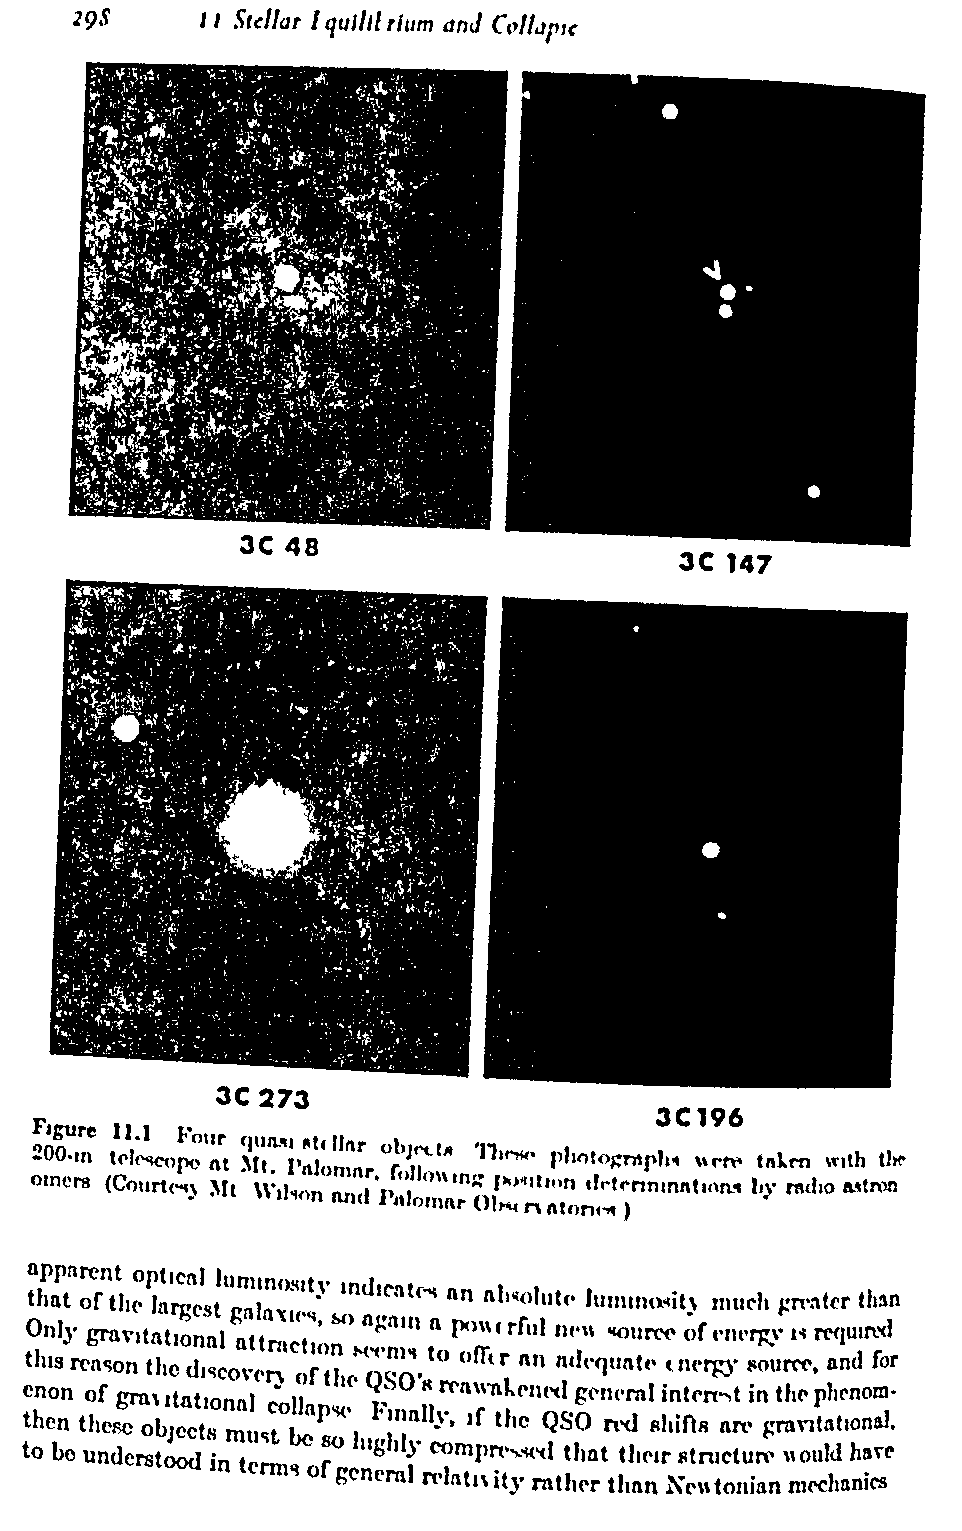
\includegraphics[
      height=0.255\textheight,
      trim=62bp 999bp 454bp 57bp,
      clip
    ]{figures/chapter11/fig11-01-source.png}
    &
    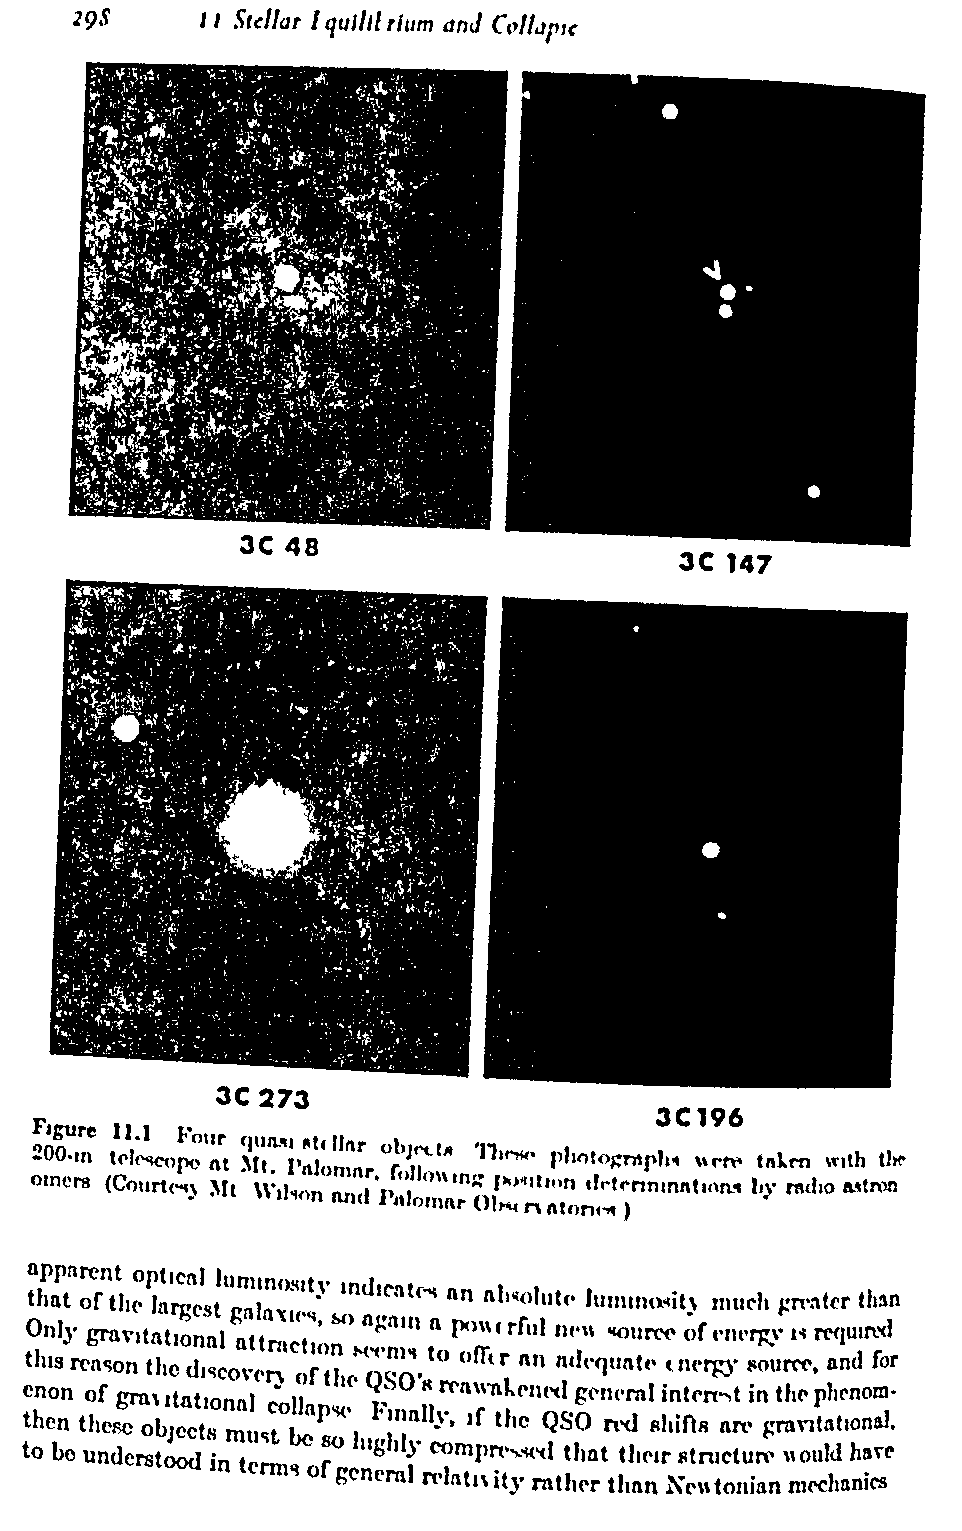
\includegraphics[
      height=0.255\textheight,
      trim=518bp 985bp 29bp 62bp,
      clip
    ]{figures/chapter11/fig11-01-source.png}
    \\
    \small\bfseries 3C 48 & \small\bfseries 3C 147
    \\[0.55em]
    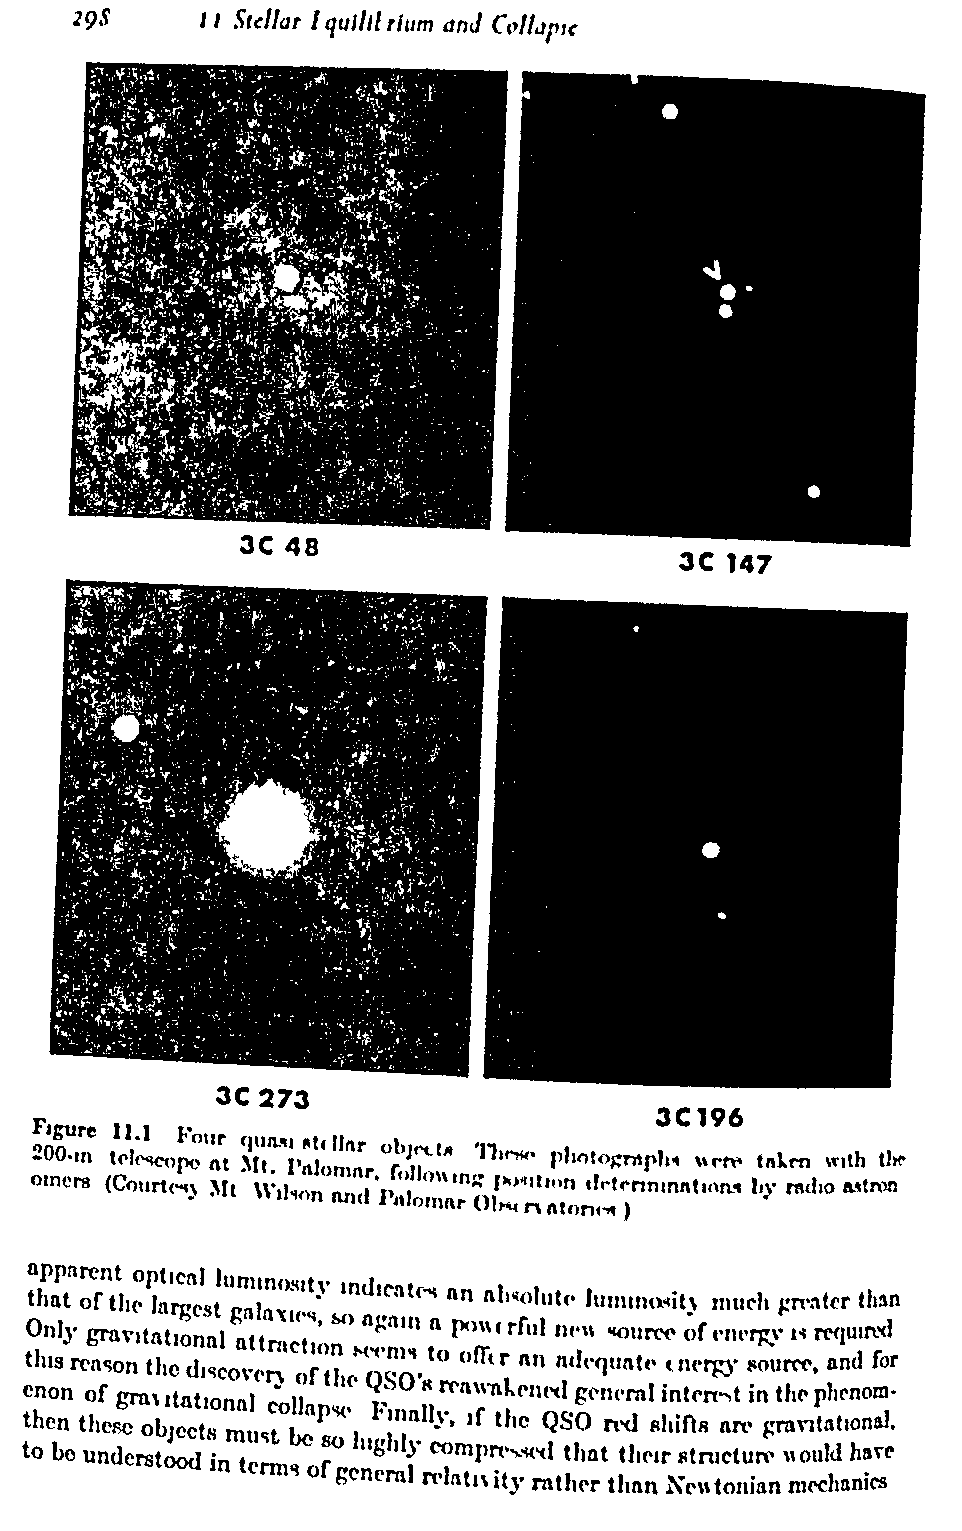
\includegraphics[
      height=0.255\textheight,
      trim=52bp 452bp 477bp 569bp,
      clip
    ]{figures/chapter11/fig11-01-source.png}
    &
    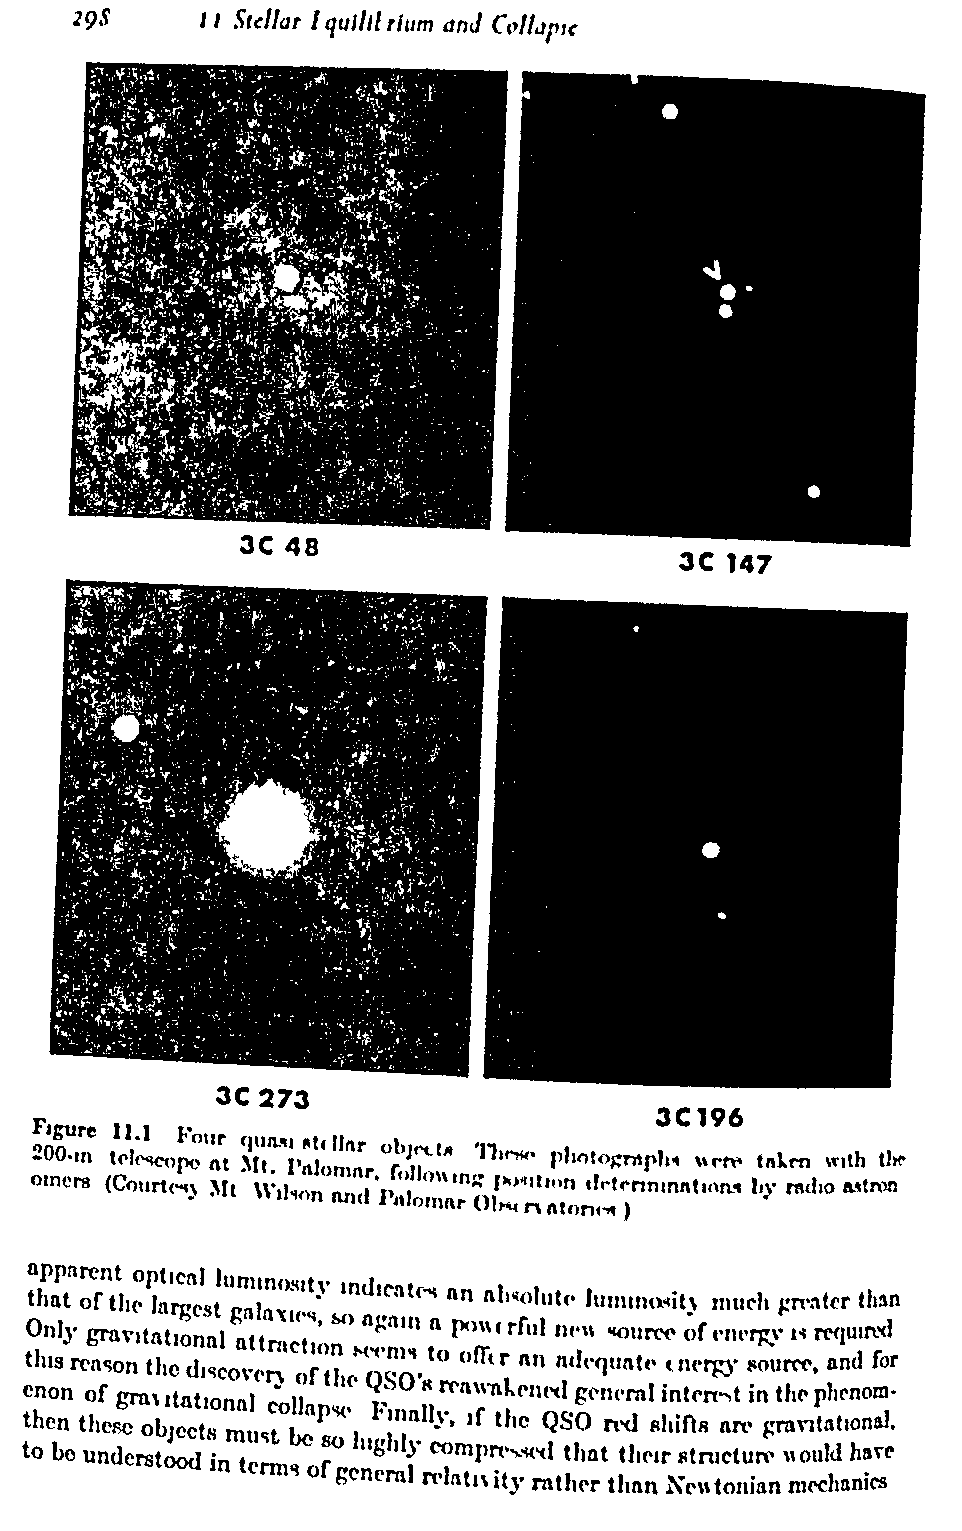
\includegraphics[
      height=0.255\textheight,
      trim=492bp 430bp 44bp 586bp,
      clip
    ]{figures/chapter11/fig11-01-source.png}
    \\
    \small\bfseries 3C 273 & \small\bfseries 3C 196
  \end{tabular}
  \caption{Four quasi-stellar objects. These photographs were taken with the
  200-in.\ telescope at Mt.\ Palomar, following position determinations by
  radio astronomers. (Courtesy Mt.\ Wilson and Palomar Observatories.)}
  \label{fig:11.1}
\end{figure}
\endgroup


The quasi-stellar objects are only the most spectacular end of a continuum of
ill-understood objects discovered in recent years, including Seyfert galaxies,
giant elliptical galaxies with powerful compact radio sources, X-ray sources,
galactic nuclei that seem in some cases to be exploding, and so on. It is not
clear what, if anything, general relativity has to do with these objects.

In the last few years a new species of astronomical exotica was
discovered---the pulsars, radio sources that pulse at regular frequencies
ranging from a few tenths of a hertz to \(30\ \mathrm{Hz}\). The pulsars are
often associated with optical and even X-ray sources that pulse at the same
rate. There appears now to be a general consensus that pulsars are the neutron
stars discovered theoretically in the 1930s, but with a rapid rate of rotation
that somehow or other produces the observed pulses.

A realistic discussion of quasi-stellar objects, galactic nuclei, pulsars,
and so on, would require that we consider the effects of radiative energy
transport, neutrino energy transport, turbulence, nuclear forces, magnetic
fields and, above all, rotation. It would also require the discussion of
massive calculations using automatic computers. In preparing this chapter, I
have tried to restrict myself to the simplest calculations, which can be
carried out analytically without too much trouble. These simple calculations
are not very useful for a detailed understanding of astronomical
observations, but they provide a valuable insight into the possible roles that
general relativity can play in astrophysical phenomena.
